%%% template.tex
%%%
%%% This LaTeX source document can be used as the basis for your technical
%%% paper or abstract. Intentionally stripped of annotation, the parameters
%%% and commands should be adjusted for your particular paper - title, 
%%% author, article DOI, etc.
%%% The accompanying ``template.annotated.tex'' provides copious annotation
%%% for the commands and parameters found in the source document. (The code
%%% is identical in ``template.tex'' and ``template.annotated.tex.'')

\documentclass[conference]{acmsiggraph}

\usepackage{authblk}
\usepackage[]{algorithm2e}

\TOGonlineid{45678}
\TOGvolume{0}
\TOGnumber{0}
\TOGarticleDOI{1111111.2222222}
\TOGprojectURL{}
\TOGvideoURL{}
\TOGdataURL{}
\TOGcodeURL{}

\title{Performance Driven Redundancy Optimization of Data Layouts for Walkthrough Applications}

%\author[1]{Zachary DeStefano\thanks{zdestefa@uci.edu}}
%\author[1]{Shan Jiang\thanks{sjiang1714@gmail.com}}
%\author[1]{Gopi Meenakshisundaram\thanks{gopi.meenakshisundaram@gmail.com}}
%\author[2]{Sung-Eui Yoon\thanks{toinsert}}
%\pdfauthor{Zachary DeStefano,Shan Jiang,Gopi Meenakshisundaram,Sung-Eui Yoon}
\pdfauthor{}
\author{}
%\affil[1]{University of California, Irvine}
%\affil[2]{KAIST}

\keywords{Data Layout Problem, Out-Of-Core Rendering, Cache Oblivious Mesh Layout, Redundant Data Layout, Walkthrough Application}

\begin{document}

%% \teaser{
%%   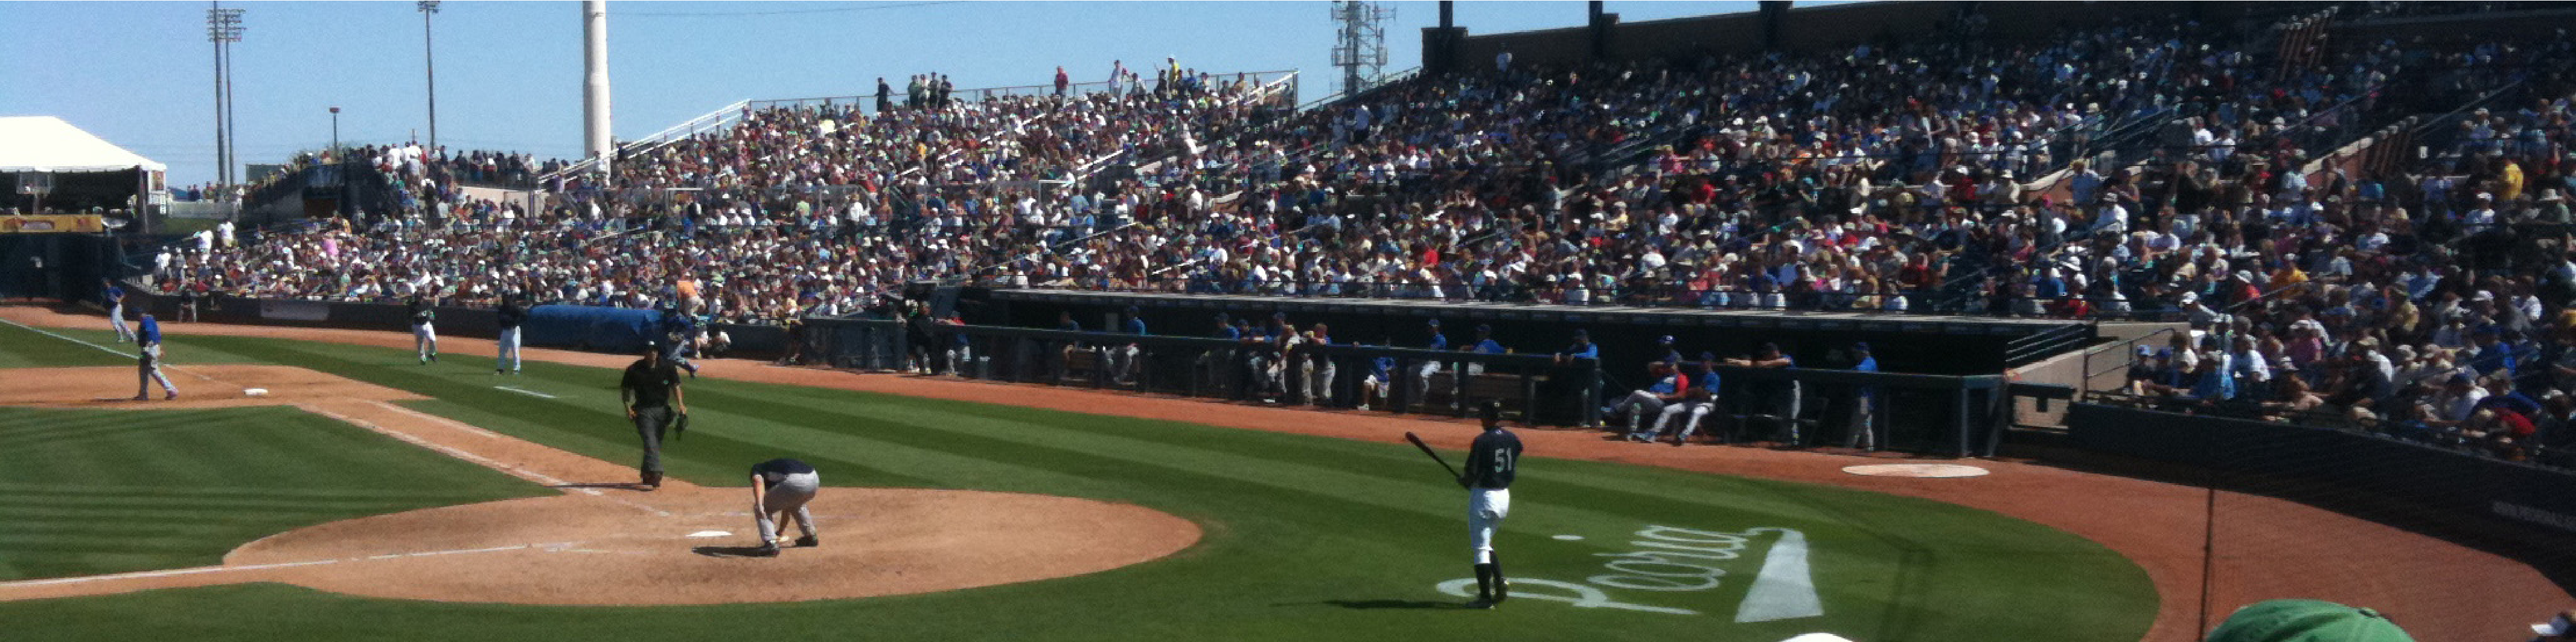
\includegraphics[height=1.5in]{images/sampleteaser}
%%   \caption{Spring Training 2009, Peoria, AZ.}
%% }

\maketitle

\begin{abstract}

Performance of interactive graphics walkthrough systems depend on the time taken to fetch the required data to render from the secondary storage to the main memory. It has been earlier established that a large fraction of this fetch time is spent on seeking the data on the hard disk. In order to reduce this seek time, redundant data storage has been proposed in the literature, but the redundancy factors of those layouts are prohibitively high.  In this paper, we develop a model for the seek time of a layout, and using this cost model, we propose an algorithm that would compute a redundant data layout with the redundancy factor that is within the user specified bounds while maximizing the performance of the system.



\end{abstract}

%\begin{CRcatlist}
%  \CRcat{I.3.6}{Computer Graphics}{Methodology and Techniques}{Graphics data structures and data types};
%\end{CRcatlist}

\keywordlist

%% Use this only if you're preparing a technical paper to be published in the 
%% ACM 'Transactions on Graphics' journal.

\TOGlinkslist

%% Required for all content. 

\copyrightspace

\section{Introduction}

\subsection{Walkthrough Rendering}

In typical walkthrough systems, data sets consisting of hundreds of millions of triangles and many gigabytes of associated data (e.g. walking through a virtual city) are quite common. Rendering such massive amounts of data requires out-of-core rendering algorithms that bring only the required data for rendering into main memory from secondary storage. In this process, in addition to the rendering speed, the data fetch speed also becomes critical for achieving interactivity, especially when we handle large-scale data. In general, data fetch speed depends on data seek time and data transfer time. Transfer time depends only on the amount of data that is transferred. Seek time is the time taken to locate the beginning of the required data in the storage device and depends on different factors depending on the storage medium. \\
\\
For a hard disk drive (HDD), its seek time depends on the speed of the disk, and the relative placement of the data units with respect to each other, also called the data layout~\cite{Rizvi10}. For a solid state drive (SSD), this seek time is usually a small constant and is independent of the location of the data with respect to each other~\cite{SSD_perf08}. An earlier work utilized this difference between SSD and HDD and designed a data layout tailored for using SSDs with the walkthrough application~\cite{ssdpaper}. There have been many other techniques utilizing SSDs for various applications~\cite{FlashVM09}. SSD, unfortunately, is not the perfect data storage and has its own technical problems, including limited number of data overwrites allowed, high cost, and limited capacity~\cite{Rizvi10}.  \\
\\
On the other hand, the HDD technology -- including disk technologies such as CDs, DVDs, and Blu-ray discs -- has become quite reliable and inexpensive thanks to their extensive verifications and testing, and is thus in widespread use.  Even for massive data sets hard disk drives (HDD) are still and will be the preferred medium of storage for the foreseeable future~\cite{Rizvi10}, mainly
because of its stability and low cost per unit. As an example, according to~\cite{pcmagarticle}, as of 2014, an HDD can cost \$0.08 per GB, while an SDD can cost \$0.60 per GB. As a result, optimizing components of walkthrough systems with HDDs is critical. In particular, addressing the seek time, the main bottleneck of accessing data from HDDs, remains the main challenge for interactive rendering of massive data sets. In this paper, we leverage the inexpensive nature of HDDs to store redundant copies of data in order to reduce the seek time. 

\subsection{Redundancy based data layouts}

In this paper, we leverage the inexpensive nature of HDDs to store redundant copies of data in order to reduce the seek time. Adding redundancy in order to improve the data access time is a classic approach, e.g., RAID~\cite{Patterson88}.  We are also not the first to consider redundancy for walkthrough applications.  Redundancy based data layouts to reduce the seek time were introduced in a recent work~\cite{singleseeklayout}, in which the number of seeks for every access was reduced to at most one unit. However, in order to achieve this property, the redundancy factor -- the ratio between the size of the data after using redundancy to the original size of the data was prohibitively high -- around 80. \\
\\
Another recent work \cite{optimizingredundancy} related a transfer volume, which dictates the data transfer time, seek time, and redundancy, and proposed a linear programming approach to optimize the data transfer and seek time in order to satisfy the total data fetch time constraint. In the process, redundancy was a hidden variable that was minimized. Unfortunately, this approach does not directly model redundancy or seek time, and thus can have unnecessary data blocks and unrealistic seek times. 

\subsection{Main Contributions}

In this paper, we propose a model for seek time based on the actual distance between the data blocks in the linear data layout. Using this model, and given the spatial proximity of the data set for a walkthrough application, we develop an algorithm to duplicate data blocks strategically to maximize the reduction in the seek time while keeping the redundancy factor within the user defined bound. We will show that our greedy solution generates both the extreme cases of data layout with redundancy, namely the no redundancy case (a simple cache oblivious mesh layout with low number of seeks) and the maximum redundancy case (a layout where seek time is at most one), as well as reasonable solutions for the redundancy factor constraints in between the extremes. We show that the implementation of our algorithm significantly reduces average delay between frames and noticeably improves the consistency of performance and interactivity.

\bibliographystyle{acmsiggraph}
\bibliography{finalPaperRefs}

\end{document}
